\documentclass[12pt]{article}
\usepackage{preamble}

\pagestyle{fancy}
\fancyhead[LO,LE]{Математическая статистика}
\fancyhead[RO,RE]{Лекции Блаженова А. В.}

\fancyfoot[L]{\scriptsize исходники найдутся тут: \\ \url{https://github.com/pelmesh619/itmo_conspects} \Cat}

\renewcommand{\thesection}{}

\begin{document}

    \tableofcontents
    \clearpage

    % begin mathstat_2025_02_11.tex





\section{Лекция 1.}

Теория вероятности изучает характеристику случайных величин, тогда как математическая статистика решает обратную задачу

Допустим, что у нас есть случайная величина, по ней мы можем найти матожидание, моменты и оценить,
какое распределение имеет случайная величина. 

\subsection{Выборки}

\Def \textbf{Выборка} - набор данных, полученных в ходе экспериментов. Тогда количество экспериментов $n$ - объем Выборки

\Defs \textbf{Генеральной совокупностью} называются все результаты проведенных экспериментов

\Defs \textbf{Выборочной совокупностью} называются наблюдаемые данные экспериментов

Не все данные экспериментов мы можем наблюдать, например, выборы, тогда опросы голосовавших - выборочная совокупность, а
результаты выборов - генеральная. Очевидно, что выборочная и генеральная совокупности могут иметь различные распределения.

\Defs Выборка называется \textbf{репрезентативной}, если ее распределение близко к распределению генеральной совокупностью

Пример - \href{https://ru.wikipedia.org/wiki/%D0%A1%D0%B8%D1%81%D1%82%D0%B5%D0%BC%D0%B0%D1%82%D0%B8%D1%87%D0%B5%D1%81%D0%BA%D0%B0%D1%8F_%D0%BE%D1%88%D0%B8%D0%B1%D0%BA%D0%B0_%D0%B2%D1%8B%D0%B6%D0%B8%D0%B2%D1%88%D0%B5%D0%B3%D0%BE}{ошибка выжившего}. Во время Второй Мировой стал вопрос, в каких местах стоит бронировать корпус самолета. Самолеты 
возвращались с пулевыми отверстиям, и интуитивно казалось, что стоит бронировать те места, которые больше
всего пострадали. Однако не были учтены те самолеты, которые не вернулись, а те, которые выжили, выжили благодаря тому, что были 
прострелены в нелетальных местах, поэтому было принято решение бронировать фюзеляж в менее пострадавших местах

В дальнейшем считаем, что все выборки репрезентативны

\DefN{1} Выборкой объема $n$ называется набор из $n$ экспериментаных данных $\vec{X} = (x_1, x_2, \dots, x_n)$ (апостериорное определение)

\DefNs{2} Выборкой объема $n$ называется набор из $n$ независимых одинаково распределенных случайных
величин $\vec{X} = (X_1, X_2, \dots, X_n)$ (априорное определение)

\subsection{Выборочные характеристики}

Можно выборку рассматривать как дискретную случайную величину с одинаковыми вероятностями $p_i = \frac{1}{n}$
и вычислить для нее математическое ожидание, дисперсию и функцию распределения

\Def Выборочным средним $\overline{X}$ называется величина $\overline{X} = \frac{1}{n} \sum_{i = 1}^n X_i$

\Defs Выборочной дисперсией $D^*$ называется величина $D^* = \frac{1}{n} \sum_{i = 1}^n (X_i - \overline{X})^2$ (или $D^* = \frac{1}{n} \sum_{i = 1}^n X_i^2 - \overline{X}^2$)

По закону больших чисел выборочное среднее будет сходиться к матожиданию

\Defs Исправленной дисперсией называется величина $S^2 = \frac{n}{n - 1} D^* = \frac{1}{n - 1}\sum_{i = 1}^n (X_i - \overline{X})^2$

\Def Выборочной функцией распределения $F^*(x)$ называется функция $F^*(x) = \frac{\text{число данных } x_i < x}{n}$

\begin{MyTheorem}
    \Ths Выборочная функция распределения поточечно сходится к теоретической функции распределения:

    \[\forall y \in \Real F^*(y) \overset{p}{\longrightarrow} F(y)\]
\end{MyTheorem}

\begin{MyProof}
    $F(y) = P(X < y)$

    $F^*_y = \frac{1}{n} \sum_{i = 1}^n I(X_i < y) \underset{\text{по ЗБЧ}}{\overset{p}{\longrightarrow}} EI(X_i < y) = P(X_i < y) = 
    P(X_1 < y) = F_{X_1}(y)$
\end{MyProof}

Усилим теорему

\begin{MyTheorem}
    \ThNs{Гливенко-Кантелли} $\sup_{x \in \Real} |F^*(x) - F(x)| \overset{p}{\longrightarrow} 0$
\end{MyTheorem}

\begin{MyTheorem}
    \ThNs{Колмогорова} $\sqrt{n} \sup_{x \in \Real} |F^*(x) - F(x)| \rightrightarrows K$ - распределение Колмогорова с 
    функцией распределения $F_K(x) = \sum_{j = -\infty}^{\infty} (-1)^j e^{-2 j^2 x^2}, \ x \in [0;\infty)$
\end{MyTheorem}

\subsection{Начальная обработка статданных}

\begin{enumerate}
    \item Ранжирование данных - упорядочиваем выборки по возрастанию. В результате получаем вариационный ряд $\vec{X} = (X_{(1)}, X_{(2)}, \dots, X_{(n)})$

    $X_{(1)} = \min X_i; \quad X_{(n)} = \max X_i$

    $X_{(i)} = i$-ая порядковая статистика

    \item Объединим повторяющиеся данные - получаем т.н. частотный вариационный ряд

    \begin{tabular}{c|c|c|c|c}
        $X_i$ & $X_{(1)}$ & \dots & $X_{(r)}$ & $\sum$ \\ 
        \hline
        $n_i$ & $n_1$ & \dots & $n_r$ & $n$ \\ 
    \end{tabular}

    Иногда часть данных отбрасывается сверху и снизу (по 5, по 10, по 5\% и так далее), чтобы сделать выборку репрезентативной

    Тогда $\overline{X} = \frac{1}{n} \sum X_i n_i$, $D^* = \frac{1}{n} \sum (X_i - \overline{X})^2 n_i$
    
    \item Чтобы уменьшить количество вычислений или сделать гистограмму, делают интервальный вариационный ряд: 
    разбиваем данные на интервалы и считаем, сколько данных $n_i$ попало в интервал. 

    Тогда $n_i$ - частота интервала $A_i$

    Есть два основные способа разбиения на интервалы: 

    \begin{enumerate}
        \item Интервалы одинаковой длины
        \item Равнонаполненные интервалы (в каждом интервале примерно одинаковое количество данных)
    \end{enumerate}

    Число интервалов $K$ такое, что $\frac{K(n)}{n} \longrightarrow 0$ и $K(n) \underset{n \to \infty}{\longrightarrow} 0$

    Обычно применяют формулу Стерджесса $K \approx 1 + \log_2 n$ или $K \approx \sqrt[3]{n}$

    Пусть получили интервальный вариационный ряд

    \begin{tabular}{c|c|c|c|c|c}
        интервалы & $[a_0; a_1)$ & $[a_1; a_2)$ & \dots & $[a_{K - 1}; a_K]$ & $\sum$ \\ 
        \hline
        частоты & $n_1$ & $n_2$ & \dots & $n_K$ & $n$ \\ 
    \end{tabular}

\end{enumerate}

\subsection{Геометрическая интерпретация данных}

% https://www.geogebra.org/calculator/rcgr7r9f

\begin{itemize}
    \item Гистограмма

    Строится ступенчатая фигура из прямоугольников, основание $i$-ого прямоугольника - интервал, 
    высота прямоугольника - $\frac{n_i}{n l_i}$, где $l_i$ - длина интервала

    \begin{center}
        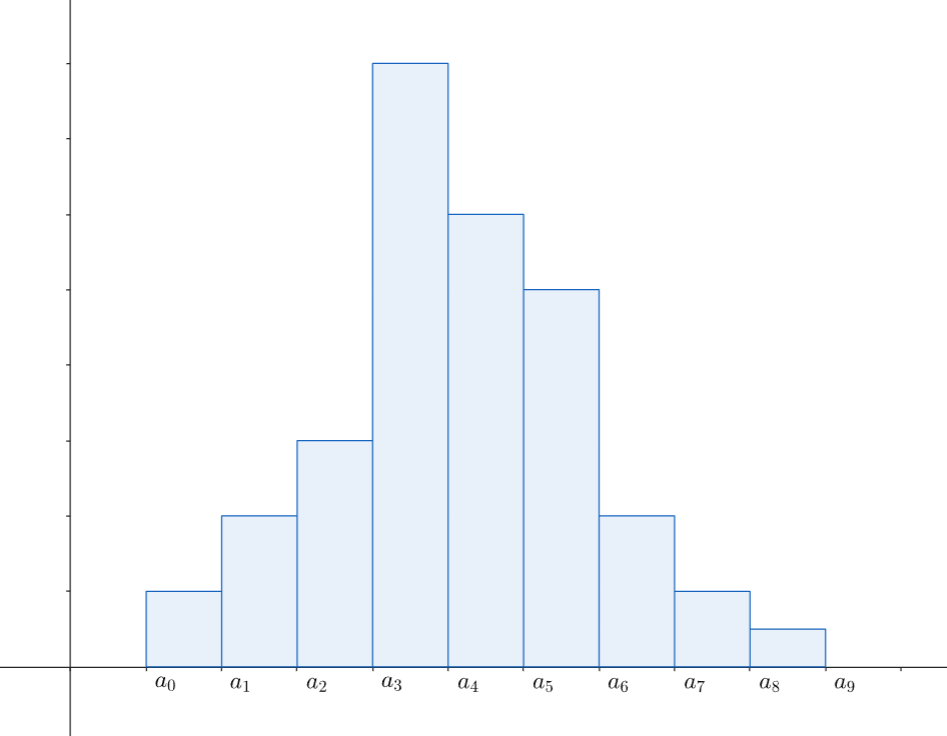
\includegraphics[width=0.7\textwidth]{mathstat/images/mathstat_2025_02_11_1}
    \end{center}

    Визуально можно сделать гипотезу, как ведет себя распределение. 

    \begin{MyTheorem}
        \Ths Гистограмма поточечно сходится к теоретической плотности
    \end{MyTheorem}

    \item Полигон

    На оси абсцисс отмечаем значения частотного вариационного ряда, по оси ординат - их частоты. 
    Получившиеся точки соединяем отрезками

    \begin{center}
        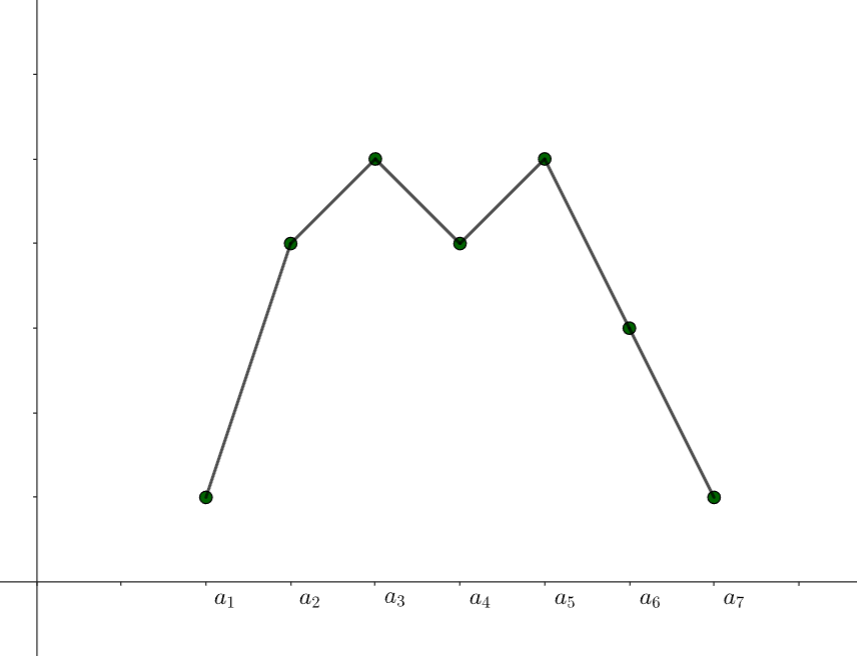
\includegraphics[width=0.7\textwidth]{mathstat/images/mathstat_2025_02_11_2}
    \end{center}

    \item Выборочная функция распределения

    На основе таблицы строится график функции распределения

    \begin{center}
        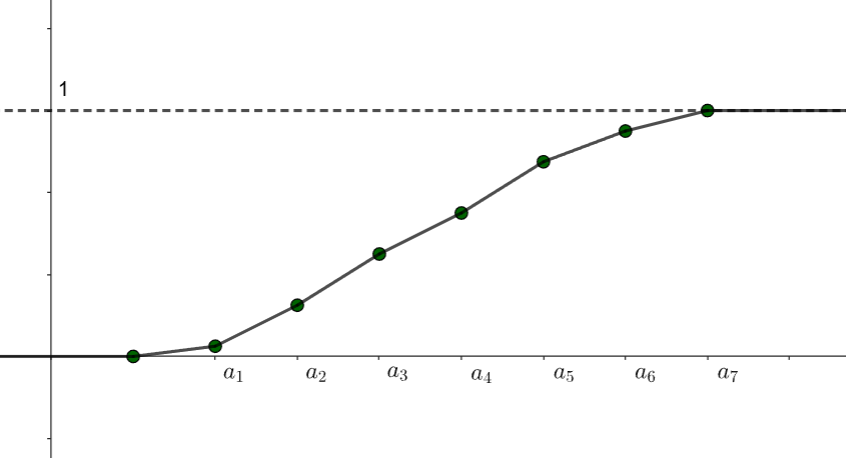
\includegraphics[width=0.7\textwidth]{mathstat/images/mathstat_2025_02_11_3}
    \end{center}

    Она может быть ступенчатой, ломаной или соединена по усмотрению

\end{itemize}





% end mathstat_2025_02_11.tex

% begin mathstat_2025_02_18.tex





\section{Лекция 2.}

\subsection{Точечная оценка}

Пусть имеется выборка $\vec{X} = (X_1, X_2, \dots, X_n)$ объемом $n$

Пусть требуется найти приближенную оценку $\theta^*$ неизвестного параметра $\theta$

Находим ее при помощи некоторой функции обработки данных $\theta^* = \theta^*(X_1, \dots, X_n)$

\Def Такая функция называется статистикой

\Defs А оценка $\theta^*$ называется точечной оценкой

\subsubsection{Свойство точечных оценок}

\begin{enumerate}
    \item Состоятельность

    \Defs Статистика $\theta^* = \theta^*(X_1, \dots, X_n)$ неизвестного параметра называется
    состоятельной, если $\theta^* \overset{p}{\longrightarrow} \theta$ при $n \to \infty$

    \mediumvspace

    \item Несмещенность

    \Defs Оценка $\theta^*$ параметра $\theta$ называется несмещенной, если 
    математическое ожидание $E \theta^* = \theta$
    
    \Notas Оценка $\theta^*$ называется асимптотически несмещенной, если 
    $E \theta^* \overset{p}{\longrightarrow} \theta$ при $n \to \infty$

    \mediumvspace

    \item Эффективность 

    \Defs Оценка $\theta^*_1$ не хуже $\theta^*_2$, если $E (\theta^*_1 - \theta)^2 \leq E (\theta^*_2 - \theta)^2$.
    Или, если $\theta^*_1$ и $\theta^*_2$ несмещенные, то $D \theta^*_1 \leq D \theta^*_2$

    \Defs Оценка $\theta^*$ называется эффективной, если она не хуже всех остальных оценок

    \Notas Не существует эффективной оценки в классе всех возможных оценок

    \begin{MyTheorem}
        \Ths В классе несмещенных оценок существует эффективная оценка
    \end{MyTheorem}

    \mediumvspace

    \item Асимптотическая нормальность

    \Defs Оценка $\theta^*$ параметра $\theta$ называется асимптотически нормальной, если 
    $\sqrt{n} (\theta^* - \theta) \rightrightarrows N(0, \sigma^2 (\theta))$ при $n \to \infty$
    
\end{enumerate}

\subsection{Точечные оценки моментов}

\Def Выборочным средним $\overline{x}$ называется величина $\overline{x} = \frac{1}{n} \sum_{i = 1}^n X_i$

\Defs Выборочной дисперсией $D^*$ называется величина $D^* = \frac{1}{n} \sum_{i = 1}^n (X_i - \overline{x})^2$

\Defs Исправленной дисперсией $S^2$ называется величина $S^2 = \frac{n}{n - 1} D^* = \frac{1}{n - 1} \sum_{i = 1}^n (X_i - \overline{x})^2$

\Defs Выборочным средним квадратическим отклонением называется величина $\sigma^* = \sqrt{D^*}$

\Defs Исправленным средним квадратическим отклонением называется величина $S = \sqrt{S^2}$

\Defs Выборочным $k$-ым моментом называется величина $\overline{x^k} = \frac{1}{n} \sum_{i = 1}^n X_i^k$

\Defs Модой $\mathrm{Mo}^*$ называется варианта $x_k$ с наибольшей частотой $n_k = \max_i (n_1, n_2, \dots, n_m)$

\Defs Выборочной медианой $\mathrm{Me}^*$ называется варианта $x_i$ в середине вариационного ряда $\begin{cases}\mathrm{Me}^* = 
X_{(k)}, & \text{если } n = 2k - 1 \\ \frac{X_{(k)} + X_{(k + 1)}}{2}, & \text{если } n = 2k\end{cases}$

\begin{MyTheorem}
    \Ths $\overline{x}$ - состоятельная месмещенная оценка теоретического матожидания $ЕX = a$

    1) $E \overline{x} = a$

    2) $\overline{x} \overset{p}{\longrightarrow} a$ при $n \to \infty$
\end{MyTheorem}

\begin{MyProof}
    1) $E \overline{x} = E\left(\frac{X_1 + \dots + X_n}{n}\right) = \frac{1}{n} \sum_{i = 1}^n E X_i = 
    \frac{1}{n} n E X_1 = E X_1 = a$

    2) $\overline{x} = \frac{\overline{x}_1 + \dots + \overline{x}_n}{n} \overset{p}{\longrightarrow} a$ 
    согласно Закону Больших Чисел
\end{MyProof}

\Nota Если второй момент конечен, то $\overline{x}$ - асимптотически нормальная оценка. По ЦПТ $\frac{S_n - n E X_1}{\sqrt{n} \sqrt{D X_1}} = \sqrt{n} \frac{\overline{x} - E X_1}{\sqrt{D X_1}} \rightrightarrows N(0, 1)$
или $\sqrt{n} (\overline{x} - E X_1) \rightrightarrows N(0; D X_1)$

\begin{MyTheorem}
    \Ths Выборочный $k$-ый момент является состоятельной несмещенной оценкой теоретического $k$-ого момента

    1) $\overline{E X^k} = E X^k$

    2) $\overline{X^k} \overset{p}{\longrightarrow} X^k$
\end{MyTheorem}

Это следует из предыдущей теоремы, если взять $X^k$ вместо $X$

\begin{MyTheorem}
    \Ths Выборочной дисперсией $D^*$ и $S^2$ являются состоятельными оценками теоретического дисперсией, при этом $D^*$ - смещенная оценка, а
    $S^2$ - несмещенная оценка
\end{MyTheorem}

\begin{MyProof}
    Заметим, что $D^* = \overline{X^2} - \overline{X}^2$

    $E D^* = E(\overline{X^2} - \overline{X}^2) = E\overline{X^2} - E (\overline{X}^2) = 
    E X^2 - E (\overline{X}^2)$

    Так как $D \overline{X} = E(\overline{X^2}) - (E \overline{X})^2$, то $E X^2 - E (\overline{X}^2) = 
    E X^2 - ((E\overline{X})^2 + D\overline{X}) = (E X^2 - EX) - D\overline{X} = D X - D \overline{X} = D X - D \left(\frac{X_1 + \dots + X_n}{n}\right) = 
    DX - \frac{1}{n^2} \sum_{i = 1}^n D X_i = DX - \frac{1}{n^2} n D X_1 = DX - \frac{1}{n} DX = \frac{n - 1}{n} DX$, то есть $D^*$ - смещенная вниз оценка

    $E S^2 = E(\frac{n}{n - 1} D^*) = \frac{n}{n - 1} \frac{n - 1}{n} DX = DX \Longrightarrow S^2$ - несмещенная вниз оценка 

    2. $D^* = \overline{X^2} - \overline{X}^2 \overset{p}{\longrightarrow} E X^2 - (E X)^2 = DX$ - состоятельная оценка

    $S^2 = \frac{n}{n - 1} D^* \overset{p}{\longrightarrow} DX$
\end{MyProof}

\Nota Отсюда видим, что выборочная дисперсия - асимптотически несмещенная оценка. Поэтому при большом (обычно не меньше 100) объеме выборке можно
считать обычную выборочную дисперсию

\subsection{Метод моментов (Пирсона)}

Постановка задачи: пусть имеется выборка объема $n$ неизвестного распределения, но известного типа,
которое задается $k$ параметрами: $\theta = (\theta_1, \theta_2, \dots, \theta_k)$. Требуется дать оценки данным
неизвестным параметрам

Идея метода состоит в том, что сначала находим оценки $k$ моментов, а затем с помощью теоретических формул
из теории вероятности даем оценки этих параметров

Пусть $\vec{X}$ - выборка из абсолютно непрерывного распределения $F_\theta$ с плотностью известного типа, 
которая задается $k$ параметрами $f_\theta (x, \theta_1, \dots, \theta_k)$

Тогда теоретические моменты находим по формуле $m_i = \int_{-\infty}^{\infty} x^i f_\theta (x, \theta_1, \dots, \theta_k) dx = h_i(\theta_1, \dots, \theta_n)$

Получаем систему из $k$ уравнений с $k$ неизвестными. В эти уравнения подставляем найденные оценки
моментов и, решая получившуюся систему уравнений, находим нужные оценки параметров

$\begin{cases}
    \overline{x} = h_1(\theta_1^*, \dots, \theta_n^*) \\ 
    \overline{x^2} = h_2(\theta_1^*, \dots, \theta_n^*) \\ 
    \dots \\
    \overline{x^k} = h_k(\theta_1^*, \dots, \theta_n^*) \\ 
\end{cases}$

\Nota Оценки по методу моментов как правило состоятельные, но часто смещенные

\Ex Пусть $X \in U(a, b)$. Обработав статданные, нашли оценки первого и второго моментов:

$\overline{x} = 2.25; \overline{x^2} = 6.75$

Найти оценки параметров $a^*, b^*$

Плотность равномерного распределения $f_{(a, b)} (x) = \begin{cases}0, & x < a \\ \frac{1}{b - a} & a \leq x \leq b, \\ 0, x > b\end{cases}$

$EX = \int_a^b x \frac{1}{b - a} dx = \frac{a + b}{2}$

$EX = \int_a^b x^2 \frac{1}{b - a} dx = \frac{a^2 + ab + b^2}{3}$

\mediumvspace

Получаем:

$\begin{cases}
    \overline{x} = \frac{a^* + b^*}{2} \\ 
    \overline{x^2} = \frac{a^*^2 + a^* b^* + b^*^2}{3} \\ 
\end{cases} \Longleftrightarrow \begin{cases}
    \frac{a^* + b^*} = 4.5 \\ 
    a^*^2 + a^* b^* + b^*^2 = 20.25 \\ 
\end{cases} \Longleftrightarrow \begin{cases}
    \frac{a^* + b^*} = 4.5 \\ 
    a^* b^* = 0 \\ 
\end{cases} \Longleftrightarrow \begin{cases}
    a^* = 0 \\ 
    b^* = 4.5 \\ 
\end{cases}$




% end mathstat_2025_02_18.tex



\end{document}

